\documentclass[12pt]{article}
\usepackage[hidelinks]{hyperref}
\usepackage[italian]{babel}
\usepackage{graphicx}
\usepackage{outlines}
\newcommand{\circumdelta}{%
  \leavevmode\vbox{
    \offinterlineskip
    \ialign{%
      \hfil##\hfil\cr
      \^{}\cr\noalign{\vskip-1ex}
      $\delta$\cr
    }
  }%
}

\begin{document}
\tableofcontents
\newpage

\section{Introduzione}
\subsection{Motivazione} 
Un linguaggio è uno strumento per descrivere come risolvere i problemi in maniera rigorosa, in modo tale che sia eseguibile da un calcolatore
Perché è utile studiare come creare un linguaggio di programmazione? 
\begin{itemize}
  \item non rimanere degli utilizzatori passivi
  \item capire il funzionamento dietro le quinte di un linguaggio
  \item domain-specific language (DSL): è un linguaggio pensato per uno specifico problema
  \item model drivern software development: modo complesso per dire UML e simili
  \item model checking
\end{itemize}


\subsection{Definizioni base} 
Un linguaggio è composto da:
\begin{itemize}
  \item lessico e sintassi
  \item compilatore: parser + generatore di codice oggetto
\end{itemize}
La generazione automatica di codice può essere dichiarativa lessico
(espressioni regolari o automa a stati finite) o sintassi(grammatiche o automa a pile).
Un automa a stati finiti consuma informazioni una alla volta, ne salva una quantità finita. Alcuni esempi di applicazione di automa a stati finiti: software di progettazione di circuiti, analizzatore lessicale, ricerca di parole sul web e protocolli di comunicazione.
\begin{figure}[h]
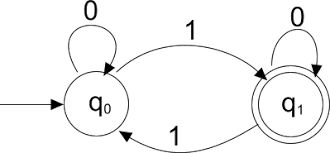
\includegraphics[scale = 0.3]{media/semplice_automa.png}
\centering
\caption{Semplice automa}
\end{figure}

\subsection{Contenuti del corso}
\begin{outline}
  \1 Linguaggi formali e Automi:
    \2 Automi a stati finiti, espressioni regolari, grammatiche libere, automi a pila, Macchine di Turing, calcolabilità
  \1 Compilatori:
    \2 Analisi lessicale, analisi sintattica, analisi semantica, generazione di codice
  \1 Logica di base:
    \2 Logica delle proposizioni e dei predicati
  \1 Modelli computazionali:
    \2 Specifica di sistemi tramite sistemi di transizione, logiche temporali per la specifica e verifica di proprietà dei sistemi (model checking), sistemi concorrenti (algebre di processi e reti di Petri)
\end{outline}

\subsection{Informazioni utili}
Parte integrante del corso:
\begin{outline}
  \1 Supporto alla parte teorica usando tool specifici.
  \2 JFLAP 7.1: http://www.jflap.org (automi/grammatiche)
  \2 Tina 3.7.5: http://projects.laas.fr/tina
  (model checking di sistemi di transizione e reti di Petri)
  \2 LTSA 3.0: http://www.doc.ic.ac.uk/ltsa
  (sistemi di transizione definiti tramite algebre di processi)
  \1 Nel resto del corso utilizzeremo un ambiente di sviluppo per
  generare parser/compilatori
  \2 IntelliJ esteso con plug-in ANTLRv4, ultima versione 1.20
  (generatore ANTLR: http://www.antlr.org/)
\end{outline}

\newpage
Libri di testo suggeriti:
\begin{outline}
 \1 J. E. Hopcroft, R. Motwani e J. D. Ullman:
Automi, linguaggi e calcolabilita’,
Addison-Wesley, Terza Edizione, 2009. Cap. 1–9
\1 A. V. Aho, M. S. Lam, R. Sethi e J. D. Ullman:
Compilatori: principi tecniche e strumenti,
Addison Wesley, Seconda Edizione, 2009. Cap. 1–5
\1 M. Huth e M. Ryan:
Logic in Computer Science: Modelling and Reasoning about
Systems,
Cambridge University Press, Second Edition, 2004. Cap. 1–3 
\end{outline}

\newpage
\section{Linguaggi regolari}
\subsection{Alfabeti}
Un \emph{alfabeto} è un insieme finito e non vuoto di simboli, comunemente indicato con $\Sigma$. Seguono alcuni esempi di alfabeti: 
\begin{outline}
  \1 $\Sigma$ = \{0,1\} alfabeto binario
  \1 $\Sigma$ = \{a,b,...,z\} alfabeto di tutte lettere minuscole
  \1 L'insieme ASCII
\end{outline}

\subsubsection{Stringhe}
Una stringa/parola è un insieme di simboli di un alfabeto, 0010 è una stringa che appartiene $\Sigma$ = \{0,1\}.
\\ La \emph{stringa vuota} è una stringa composta da 0 simboli.
\\ La lunghezza della stringa sono il numeri di caratteri che la compongono (non devono essere unici). La sintassi per la lunghezza di una stringa w è $|w|$, quindi $|001|$ = 3 oppure $|\epsilon| = 0$ (nota bene, $\epsilon \ne 0$ ma è di lunghezza 0).

\subsubsection*{Potenze di un alfabeto}
Se $\Sigma$ è un alfabeto si può esprimere l'insieme di tutte le stringhe di una certa lunghezza con una notazione esponenziale: $\Sigma^k$ denota tutte le stringhe di lunghezza k con simboli che appartengono a $\Sigma$. \\
Per esempio: 
\\ $\Sigma^1$ = \{0,1\} 
\\ $\Sigma^2$ = \{00, 01, 10, 11\}
\\ $\Sigma^2$ = \{000, 001, 010, 011, 100, 101, 110, 111\}
\\ L'insieme delle stringhe meno quella vuota è segnato come $\Sigma^+$, mentre l'insieme che include la stringa vuota è $\Sigma^*$,

\subsubsection{Concatenazione di stringhe}
Siano x e y stringhe, dove i è la lunghezza di x e j è la lunghezza di y, la stringa xy è la stringa risultata dalla concatenazione delle stringhe xy di lunghezza i+j.

\subsection{Definizione di linguaggio}
Un insieme di stringhe a scelta L $\subseteq\Sigma^*$ si definisce linguaggio su $\Sigma$. 
\\ Un modo formale per definire un alfabeto è il seguente \{w $|$ enunciato su w\}, che si traduce in "w tale che enunciato su w".
\\ $\{0^n 1^n | n \ge 1 \}$ si traduce in "l’insieme di 0 elevato alla n, 1 alla n tale che n è maggiore o uguale a 1" 

\newpage
\section{Automa a stati finiti}
Un automa a stati finiti deterministico consiste in: 
\begin{enumerate}
  \item Un insieme di stati finiti Q
  \item Un insieme di simboli di input, $\Sigma$
  \item Una funzione di transizione, che prende in input uno stato e un simbolo e restituisce uno stato. Tale funzione è spesso indicato con $\delta$ ed è usata per rappresentare i archi nella rappresentazione grafica. Ovvero sia \emph{q} uno stato, \emph{a} un input allora $\delta$(q,a) è lo stato \emph{p} tale che esista un arco da q a p.
  \item Uno stato iniziale (naturalmente che appartiene a Q)
  \item Un insieme di stati accettati finali F. Questo è un sottoinsieme di Q.
\end{enumerate}
Un automa a stati finiti deterministico è spesso chiamato con l'acronimo DFA e viene può essere rappresentato nella seguente maniera concisa: 
\[A = (Q, \Sigma, \delta, q\textsubscript{0}, F)\]
Dove A rappresenta il DFA.

\subsection{ Elaborazione di stringhe }
Per elaborare una stringa è si definisce lo stato iniziale, quello finale e una serie di regole di transizione per poterci arrivare. 
Se dovessi decodificare la stringa 01 il DFA risulterebbe: 
\[A = (Q=\{q1,q2,q3\}, \{0,1\}, \delta, q\textsubscript{0}, \{q1\})\]
I stati sono i sequenti: 
\\ $\delta(q\textsubscript{0},1)=q\textsubscript{0}$: leggo come primo stato 1, nessun progresso fatto
\\ $\delta(q\textsubscript{0},0)=q\textsubscript{2}$: leggo come primo stato 0, posso andare avanti e cercare un 1
\\ $\delta(q\textsubscript{2},1)=q\textsubscript{1}$: leggo 1 dopo lo 0, ho trovato la stringa
\\ $\delta(q\textsubscript{2},0)=q\textsubscript{2}$: leggo 0 dopo lo 0, non ho fatto progresso
\\ Nota bene: questa è una notazione arbitraria del libro, q1 e q2 si possono invertire.

\subsubsection{ Notazioni semplici per DFA }
\subsubsection*{ Diagramma di transizione }
Dato un DFA $A = (Q, \Sigma, \delta, q\textsubscript{0}, F)$ un suo diagramma di transizione è composto da: 
\begin{outline}
  \1 Ogni stato Q è un nodo 
  \1 Ogni funzione $\delta$ è una freccia
  \1 La freccia Start che denota il primo input 
  \1 Gli stati accettati F hanno un doppio cerchio
\end{outline}
\begin{figure}[h]
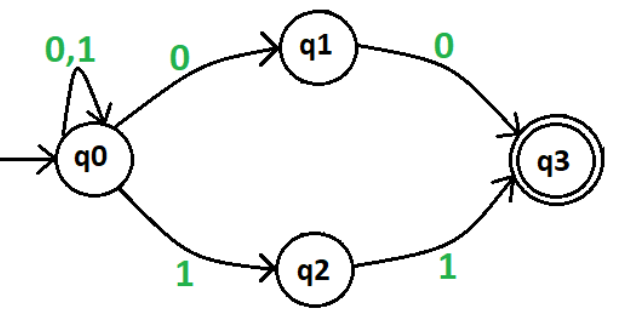
\includegraphics[scale = 0.3]{media/diagramma_stato.png}
\centering
\caption{Diagramma di transizione}
\end{figure}

\subsubsection*{ Tabelle di transizione }
Una tabella di transizione è costituita nelle riga dalle funzioni $\delta$ e nelle colonne dagli input. Ogni incrocio equivale a uno stato della funzione $\delta$ con un input generico \emph{a}.

\begin{table}[h]
\centering
\begin{tabular}{c | c | c}
& 0 & 1 \\
\hline
$\rightarrow$  q\textsubscript{0} & q\textsubscript{2} & q\textsubscript{0} \\
$*$q\textsubscript{1} & q\textsubscript{1} & q\textsubscript{1} \\
q\textsubscript{2} & q\textsubscript{2} & q\textsubscript{1} \\
\end{tabular}
\caption{Esempio di tabella}
\end{table}
La freccia è lo start e l'asterisco è lo stato finale.

\subsubsection{ Estensione della funzione di transizione di stringhe }
Allo scopo di poter seguire una sequenza di input ci serve definire una funzione di transizione estesa. Se $\delta$ è una funzione di transizione, chiameremo \circumdelta\space la sua funzione estesa.
La funzione estesa prende in input \emph{q} e una stringa \emph{w} e ritorna uno stato \emph{p}. 
\\ Ogni stato viene calcolato grazie allo stato esteso precedente: \[\circumdelta(\emph{q,w}) = \delta(\circumdelta(\emph{q,x}), \emph{a})\]
\subsubsection*{Esempio}
L = \{ w $|$ w ha un numero pari di 0 e di 1 \}
\\ Nota bene: 0 è pari quindi conta come stato accettato, ed è l'unico stato accettato. 
\\ \hspace*{0.4cm} q\textsubscript{0}: 0 e 1 sono pari
\\ \hspace*{0.4cm} q\textsubscript{1}: 0 pari 1 dispari
\\ \hspace*{0.4cm} q\textsubscript{2}: 1 pari 0 dispari
\\ \hspace*{0.4cm} q\textsubscript{3}: 0 dispari 1 dispari
\[A = (\{q1,q2,q3,q4\}, \{0,1\}, \delta, q\textsubscript{0}, \{q\textsubscript{0}\})\]


\end{document}

